
\section{Feedback Training}
After determining the amplitude thresholds, the subject was trained in understanding the sensory feedback. Depending on which group the subject was allocated to, the subject was either trained in understanding the spatial or amplitude scheme first. The structure of the training was, however, the same. The feedback training was divided into two phases: familiarization and reinforced learning. These phases will be presented in the following sections.

\subsection{Familiarization} \label{sec:meth:FBtrainingFam}
In the familiarization phase, the subject was presented with the sensation of 12 different grid squares and 12 grid squares indirectly, while observing which grid location corresponded to which sensation. This was carried out by the investigators by moving the cursor seen in \figref{fig:gridmap_FBfam} with the arrow keys on the keyboard. One press with an arrow key would move the cursor in a different grid square in the direction relative to the arrow key pressed. Pressing return would place the cursor in the staring point (the third grid square in the first row). The order of which grid square the cursor would be moved to can be seen in \figref{fig:gridmap_FBfam}. After reaching a designated square, the cursor would be reset to the starting point. When moving the cursor to a grid square not adjacent to the staring point, the feedback from the transition grid squares would be felt. This transition is transferable to practical proportional prosthetic control/feedback, where the transition from rest to an outer prosthetic position is apparent. When moving the cursor to the grid squares 9, 10, 11 and 12, representing combined DoF positions, the direct route (moving fully in one direction and then the other) was used. In the familiarization phase, the cursor would be moved fully horizontally and then vertically. This enabled stimulations relative to all grid square to be included in the familiarization, without setting all grid squares to be designated targets. This design was chosen due to the single DoF direction being assessed to be most important to get familiar with, and to save time while still exposing the subject to all possible stimulations. Time spend in designated squares was approximately four seconds and time spend in transition squares was approximately two seconds.

\begin{figure}[H]                 
	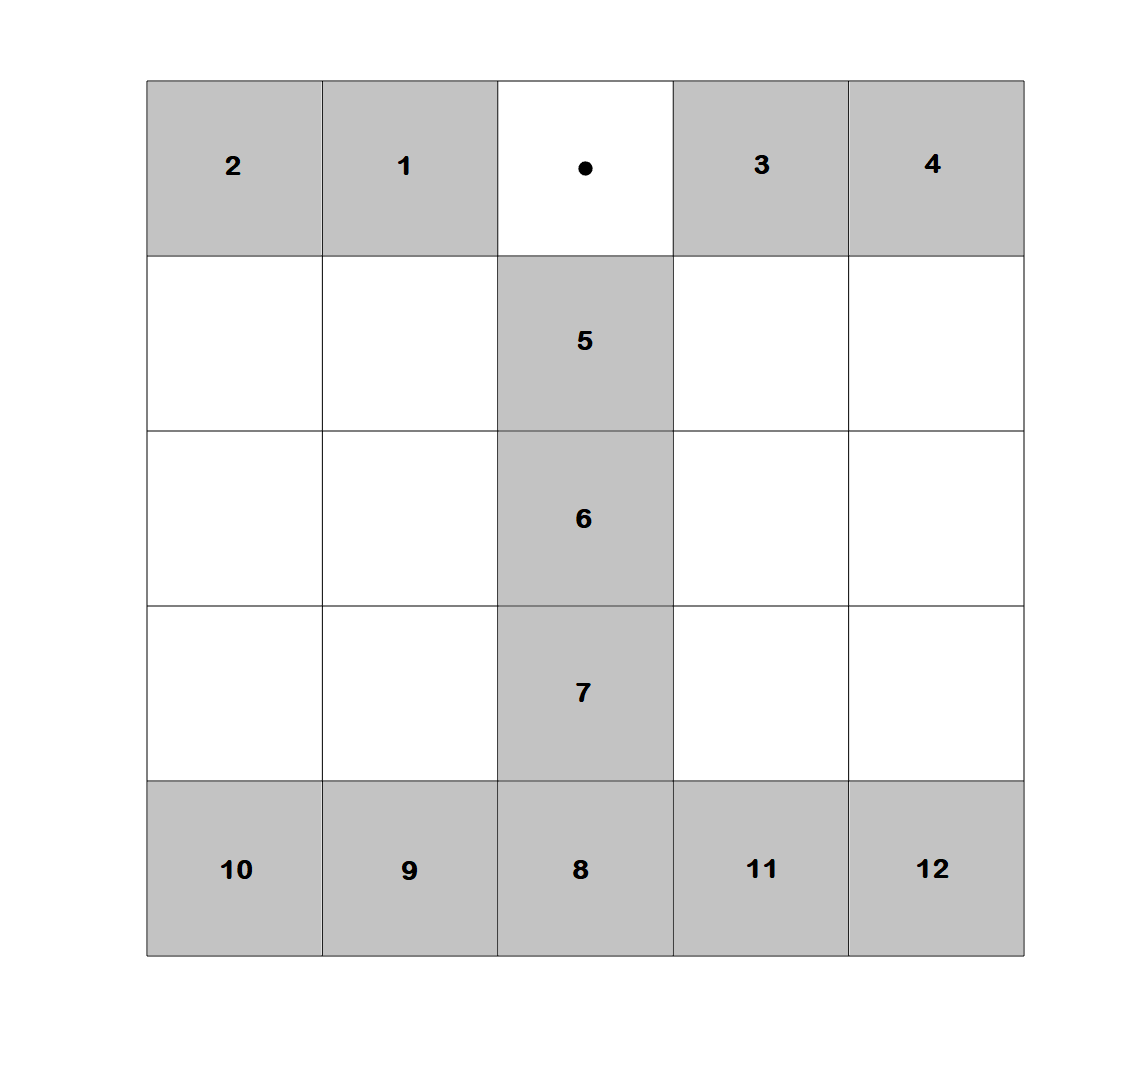
\includegraphics[width=0.55\textwidth]{figures/gridmap_FBfam}  
	\caption{Illustration of the order the cursor would be moved to which grid squares in. The numbered grey squares are designated squares. After reaching a designated square, the cursor would be reset to staring position (the grid square the cursor is located in).}
	\label{fig:gridmap_FBfam} 
\end{figure}

\subsection{Reinforced Learning} \label{sec:meth:FBtrainingRe}
The reinforced learning phase consisted of two blocks, in which all grid squares were designated squares. When a designated square was reached the investigator asked the subject about the location of the cursor. If the subject answered incorrectly, the investigator would reveal the actual location of the cursor. The stimulation related to the designated would be active until the subject answered. Afterwards, the cursor would be reset to the starting point. \\
The difference between the two blocks was the order and path to the designated squares, which was predetermined by the investigators. The blocks were, however, identical for all subjects. The path to a designated square was the direct route. However, which direction that would be moved in first was predetermined by the investigators. Thus, the transition stimulations would be felt by the subject before the designated was reached. This design was implemented to avoid bias in being accustomed to always receiving stimulation related to the same DoF first before the other. Time spend in transition squares was approximately two seconds. 